\documentclass[a4paper]{jpconf}
%\bibliographystyle{iopart-num}
%\usepackage{citesort}
\usepackage{graphicx}

\begin{document}
\title{A Geant4 physics list for spallation and related nuclear physics applications 
based on INCL and ABLA models}

\author{A Heikkinen$^1$, A Boudard$^2$, P Kaitaniemi$^{1,2}$ and G Folger$^3$}
\address{$^1$ Helsinki Institute of Physics, P.O. Box 64, FIN-00014 University of Helsinki, Finland}
\address{$^2$ CEN-Saclay, CEA-IRFU/SPhN, 91 191 Gif sur Yvette, France}
\address{$^3$ European Organization for Nuclear Research (CERN), Switzerland}

\ead{aatos.heikkinen@cern.ch}

\begin{abstract}
A new Geant4 physics list is prepared for nuclear physics applications
in the domain dominated by spallation.
The C++ translation of original Fortran INCL intra-nuclear 
cascade and ABLA fission/de-excitation codes 
are used in the physics list.
The INCL model prepared is well established for targets heavier than Aluminium
and projectile energies from 150 MeV up to 2.5 GeV - 3 GeV.
%Validity of the Geant4 physics list is demonstrated from 
%the perspective of accelerator driven systems and EURISOL project, %PK::: uncomment material added
%especially with the neutron double differential cross sections and residual nuclei production.
Validity of the new Geant4 physics list is demonstrated, 
and the neutron double differential cross sections and residual nuclei production discussed.
Foreseen improvements of the physics models for the treatment of light targets (Carbon - Oxygen)
and light ion beams (up to Carbon) are discussed.
%An example application utilizing the physics list is introduced. %PK::: uncomment if material added
\end{abstract}

\section{Introduction} \label{sec:intro}
This paper is focused on issues relevant to Geant4 \cite{geant4} simulation of nuclear physics applications,
modelling of spallation reactions, and validating neutron production and fragmentation.

% Material: http://users.ictp.it/~pub_off/lectures/lns012/Kadi_002.pdf
Our motivation is to develop Geant4 simulation tools for European Isotope Separation On-Line
Radioactive Ion Beam Facility (EURISOL project) \cite{eurisol} and 
Accelerator Driven Systems (ADSs) \cite{ads}. 
The main goal of accelerator driven sub-critical reactor development
is to provide a facility dedicated to the transmutation of long lived
isotopes issued from the nuclear industry (mainly nuclear wastes from
nuclear power plants).  Spallation is also used for the production
of intense neutron sources of wide energy spectra which are useful for
material study and fundamental measurements.

To this aim we present a new Geant4 physics list, 
based on INCL \cite{incl} intra-nuclear cascade model and ABLA de-excitation model \cite{abla, abla1, abla2} in Geant4 9.2. 
This physics list can be used to simulate the main components of an ADS system: accelerator, spallation
target and sub-critical core.

This paper is organized as follows.
Section~\ref{sec:list} briefly summarises the concept of Geant4 physics list.
Geant4 9.2 models intra-nuclear cascade INCL or Liege cascade, and ABLA evaporation-fission model
applied in this work are introduced in Section~\ref{sec:models}, 
while Section~\ref{sec:newlist} documents the details of physics list implementation.
%Secctio~\ref{sec:example} describes an example application utilizing the new physics list
%for the use case of spallation reaction study.
Physics performance is demonstrated in Section~\ref{sec:performance},
and status of carbon projectiles is given in Section~\ref{sec:carbon}. 
Section~\ref{sec:conclusion} concludes with outline of future developments.

\section{Geant4 physics lists}\label{sec:list}

A unique feature of Geant4 is to decouple physics models, cross sections, and processes
using abstract interfaces, and manage the usage of different options with so-called the physics lists:
\begin{itemize}
\item Concept provides transparent access to various physics models.
\item The Geant4 physics system can be easily extended with new models and cross sections.
\item Physics lists allow users to find a good balance between various goals 
(e.g. CPU time requirements vs. accuracy of results).
\end{itemize}

Often optional models are available with specific strengths and limitations, 
so physics lists concept is used to provide optimal set of functionality for specific use case.

\section{INCL and ABLA models in Geant4} \label{sec:models}

INCL and ABLA models are cast into independent Fortran based Monte Carlo codes 
INCL4.2 \cite{incl} and ABLA v3 \cite{abla}.
Recently these implementations have been translated into C++ and codes distributed
as part of the Geant4 toolkit \cite{pk08bProceedings}. 
The first beta release of INCL 4.2 and ABLA v3 was in Geant4  9.1 (December 2007)~\cite{g4site}.
Currently the INCL and ABLA versions in Geant4 are straightforward
Fortran to C++ translations.
Table~\ref{tab:inclabla} summarises the key features of these models.

\begin{center}
\begin{table}[h]
\caption{\label{tab:inclabla}Summary of key features of INCL and ABLA models in Geant4~\cite{pk08bProceedings}.}
%\footnotesize\rm
\centering
\begin{tabular}{@{}*{7}{l}}
\br
{\bf INCL4.2}& \\
\mr

Projectiles & Protons, neutrons, pions ($\pi^-$, $\pi^0$, $\pi^+$)\\
& d, t, $^3{\rm He}$, $\alpha$\\
Energy range & $\sim$150~MeV -- $\sim$3GeV \\
Target nuclei & Carbon -- Uranium \\
Model features&  Stand alone mode with built in random number generation\\
& No ad hoc parameters \\
& Woods-Saxon nuclear potential \\
& Coulomb barrier \\
& Pauli blocking \\
& non-uniform time step \\
& $\pi$ and $\Delta$ production cross sections \\
& $\Delta$ decay \\

{\bf ABLA v3}& \\
\mr
Supported input & Exited nuclei \\
Model features & Fission \\
& Evaporation of p, n, and $\alpha$\\
Output particles & Fission products, residual nuclei, p, n, $\alpha$\\
\mr
\end{tabular}
\end{table}
\end{center}

\section{A new Geant4 physics list {\tt QGSP\_\-INCL\_ABLA}}\label{sec:newlist}

We have implemented a new physics list called {\tt QGSP\_\-INCL\_ABLA} with
spallation physics in mind. 
The list is based on the widely used {\tt QGSP\_BERT} physics list.
The new physics list uses INCL and ABLA models for proton,
neutron, pion, deuteron, triton, He-3 and alpha inelastic interactions in the energy range 0~-~3~GeV.
Above 3~GeV threshold Geant4 Bertini cascade model is used and above 15~GeV QGSP high energy model. However, since this list is intended for
spallation and ADS applications we have not optimized the physics
performance for energies higher than 3~GeV. 
Key features of {\tt QGSP\_INCL\_ABLA} physics list are summarised in Table~\ref{tab:list}.

\begin{center}
\begin{table}[h]
\caption{\label{tab:list}Summary of {\tt QGSP\_\-INCL\_ABLA} physics list~\cite{pk08bProceedings}.}
%\footnotesize\rm
\centering
\begin{tabular}{@{}*{7}{l}}
\br
Models&Description\\
\mr
Electromagnetic physics & Geant4 standard EM\\
Spallation modelling & INCL cascade with ABLA fission and evaporation (E$<$3~GeV)\\
High energy model & Bertini cascade (E $>$ 3~GeV), QGSP (E$>$15~GeV)\\
\br
{\bf Use-cases} &  \\
 & Spallation studies \\
                    & Accelerator driven systems  \\
                   & Fragment production \\
                   & Neutron production \\
\br
\end{tabular}
\end{table}
\end{center}
The class reference documentation of the INCL/ABLA models is produced
using Doxygen \cite{doxygen} documentation generator (see Fig.~\ref{fig:doxygen}). 
It allows us to produce full documentation of the class structure complete with usage
instructions, class diagrams, detailed descriptions of all methods and
code listings.

\begin{figure}[h]
\begin{center}
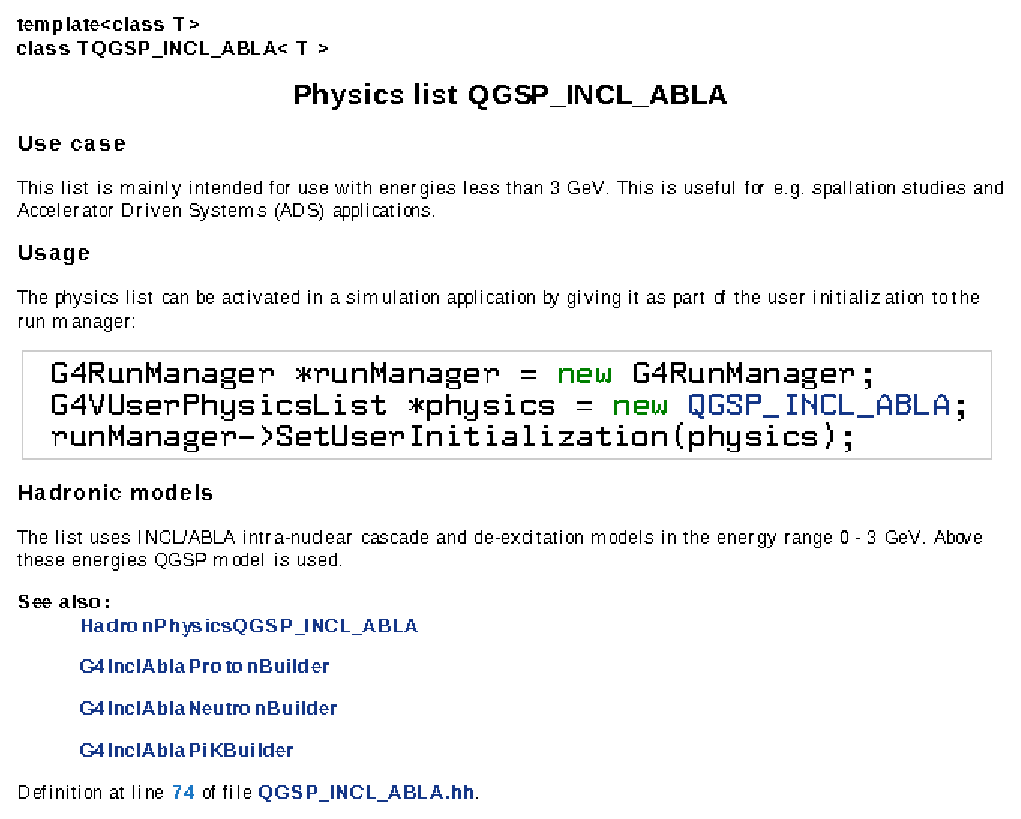
\includegraphics[scale=0.70]{poster/images/inclAblaDoc.eps}
\caption{Doxygen documentation of Geant4 {\tt QGSP\_\-INCL\_ABLA} physics list is provided.}
\end{center}
\label{fig:doxygen}
\end{figure}

\section{Physics performance}\label{sec:performance}
Extensive validation has been performed to ensure the quality of INCL and ABLA models and correctness
of Fortran to C+ translation. 
% Neutron production is the main method of validation
Particularly double-differential neutron production cross sections of
Al - Pb targets bombarded by 0.8 - 1.6 GeV protons have been
investigated with simulations and comparison with accurate experimental data
from~\cite{data}.
% and fragment production comes after that
In addition to neutron production also fragment production has been
compared against data from Refs~\cite{carbone, gsifragments}.

%% Particularly fragmentation of C - Pb targets bombarded with 0.8 - 1.6 GeV protons has been investigated
%% with simulations and results compared with experimental data~\cite{carbone, gsifragments}.
%% In addition to mass number distributions neutron production double differentials
%% have been compared with accurate data from~\cite{data}.

In case of light cascade remnant nuclei de-excitation Fermi break-up
model is more appropriate choice than ABLA.
We have made this functionality available through the INCL Geant4 interface.
%To achieve this we have
%introduced a selection rule that chooses Geant4 Fermi break-up for remnants with
%mass number smaller than 13 and ABLA for remnants with mass number 13
%or more.
Currently, INCL interface uses Geant4 Fermi break-up~\cite{g4fermi} for
remnant nuclei lighter than A = 13 and ABLA for heavier elements.


For example, comparison of the fragment production results for reaction p(1.0 GeV) + C 
calculated using INCL and ABLA, INCL with Fermi break-up and
Geant4 Bertini cascade are shown in Fig.~\ref{fig:breakc}.
Table~\ref{tab:validation} summarises the validations reported in this paper.

\begin{figure}[h]
\begin{minipage}{9.0cm}
%\begin{center}
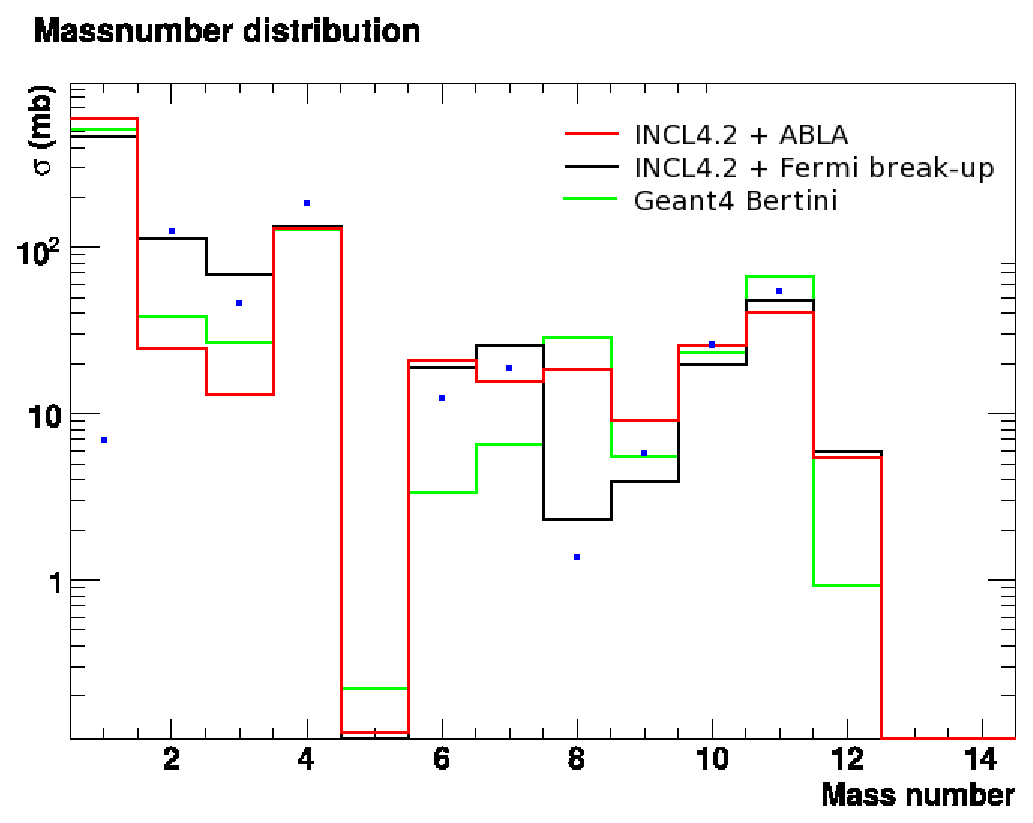
\includegraphics[width=1.0\textwidth]{poster/images/masses2.eps}
%\end{center}
%\caption{\label{label}Figure caption .}
\end{minipage}\hspace{2pc}%
\begin{minipage}{6cm}
\caption{\label{fig:breakc}Comparison of mass number distributions from p(1.0~GeV) + C reaction,
given by INCL4.2 cascade with ABLA evaporation 
and with standard Geant4 Fermi break up model against data from \cite{carbone}.
Also, results from Geant4 Bertini cascade with internal fragmentation model are shown. }
\end{minipage} 

\end{figure}


\begin{center}
\begin{table}[h]
\caption{Summary of Geant4 INCL ABLA validations.}
%\footnotesize\rm
\centering
\begin{tabular}{@{}*{7}{l}{l}}
\br
Validation & Configuration & Figure \\
\mr
{\bf Fragmentation} & & \\
 & p(1.0 GeV) + C & Fig.~\ref{fig:breakc} \\
 &  p(1.0~GeV) + $^{208}{\rm Pb}$ & Figs.~\ref{fig:fragpb} and \ref{fig:fragisotopes} \\
\br
{\bf Neutron production} &  & \\
 & p(1.2 GeV) + Al $\rightarrow$ n + X & Fig.~\ref{fig:neutronAl} \\
 & p(0.8 GeV) + Fe $\rightarrow$ n + X & Fig.~\ref{fig:neutron08Fe} \\
 & p(1.6~GeV) + Fe $\rightarrow$ n + X & Fig.~\ref{fig:neutronFe} \\
 & p(1.6~GeV) + Pb $\rightarrow$ n + X & Fig.~\ref{fig:neutronPb} \\
\br
\end{tabular}
\label{tab:validation}
\end{table}
\end{center}

\begin{figure}[h]
\begin{center}
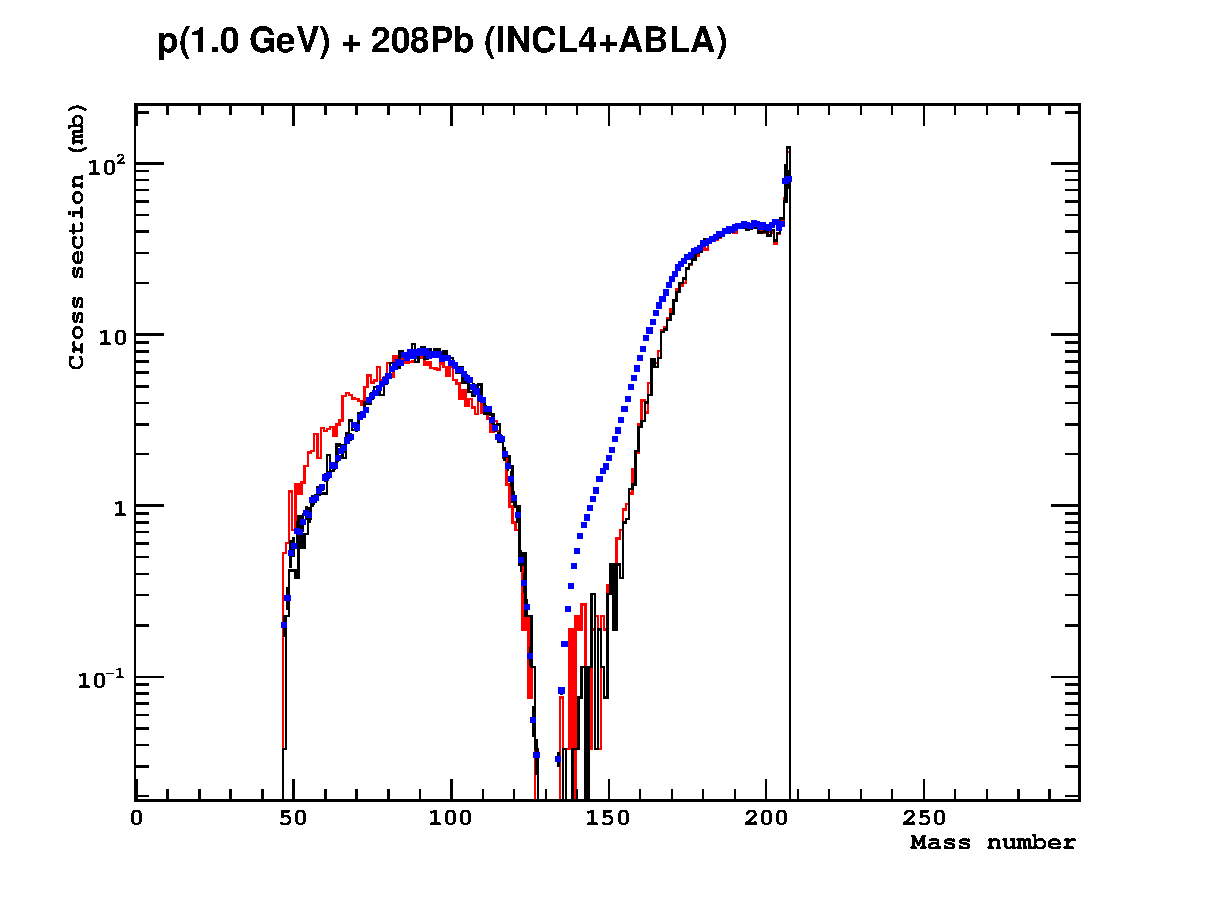
\includegraphics[scale=0.80]{images/proton1000MeVPb.eps}

\caption{\label{fig:fragpb}Mass distribution of fragments  for p(1.0~GeV) + $^{208}{\rm Pb}$ interaction 
using the INCL and ABLA  models.
Histograms are the results from the original FORTRAN version (black) 
and new C++ implementation (red). Data is from Ref.~\cite{gsifragments}
(the reason for the difference between the C++ and FORTRAN versions is under investigation).}
%(the reason for the difference
%between the fortran version and the C++ version in the fission part is
%not yet fully understood... (which means in clear for us that there is
%a mistake in the coding)).}

\end{center}
\end{figure}

\begin{figure}[h]
\begin{center}
%Isotope production:
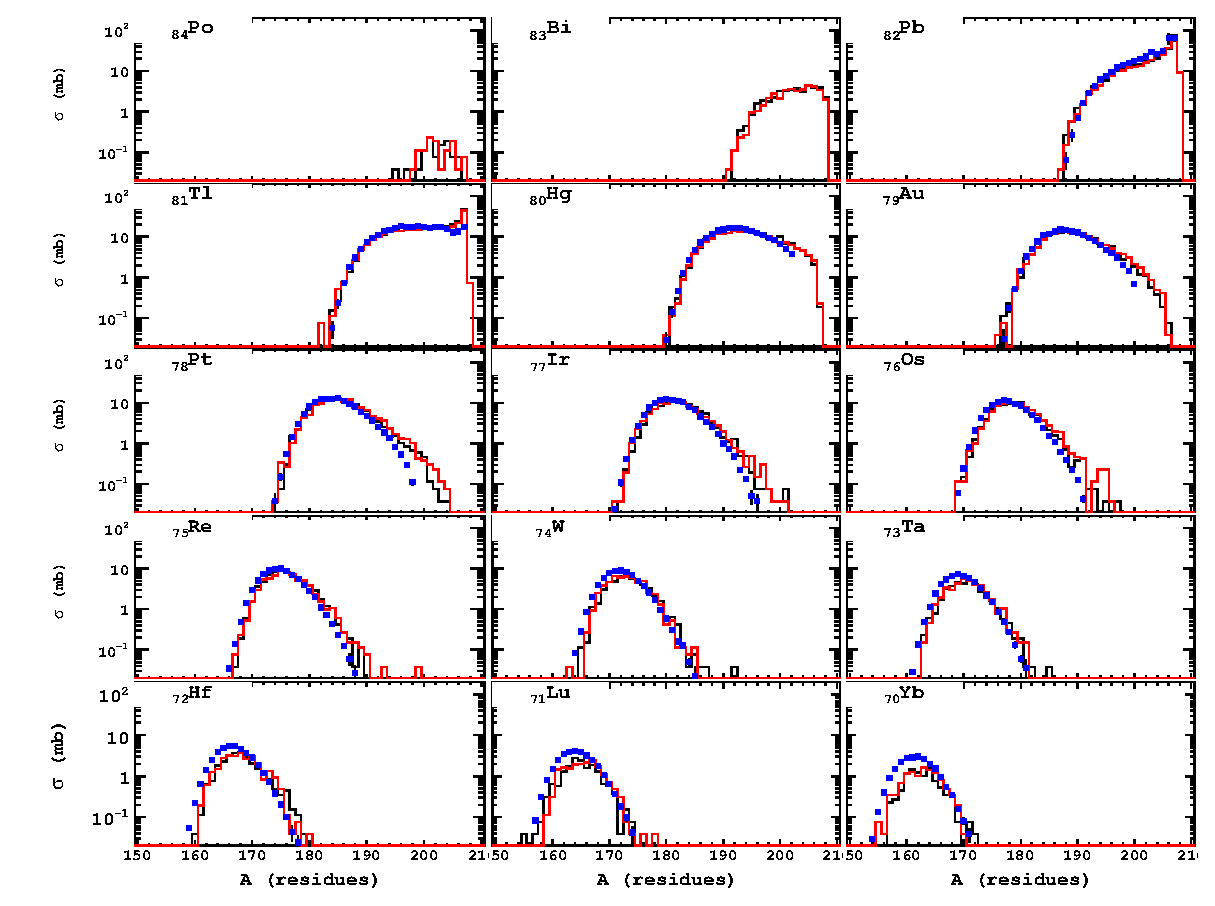
\includegraphics[scale=0.80]{poster/images/pPbIsotopes.eps}

\caption{\label{fig:fragisotopes}Fragment production of the INCL and ABLA  models 
for p(1.0~GeV) + $^{208}{\rm Pb}$ interaction.
Histograms are the results from the original FORTRAN version (black)
and new C++ implementation (red). Data is from Ref.\cite{gsifragments}.}

\end{center}
\end{figure}


\begin{figure}
\begin{center}
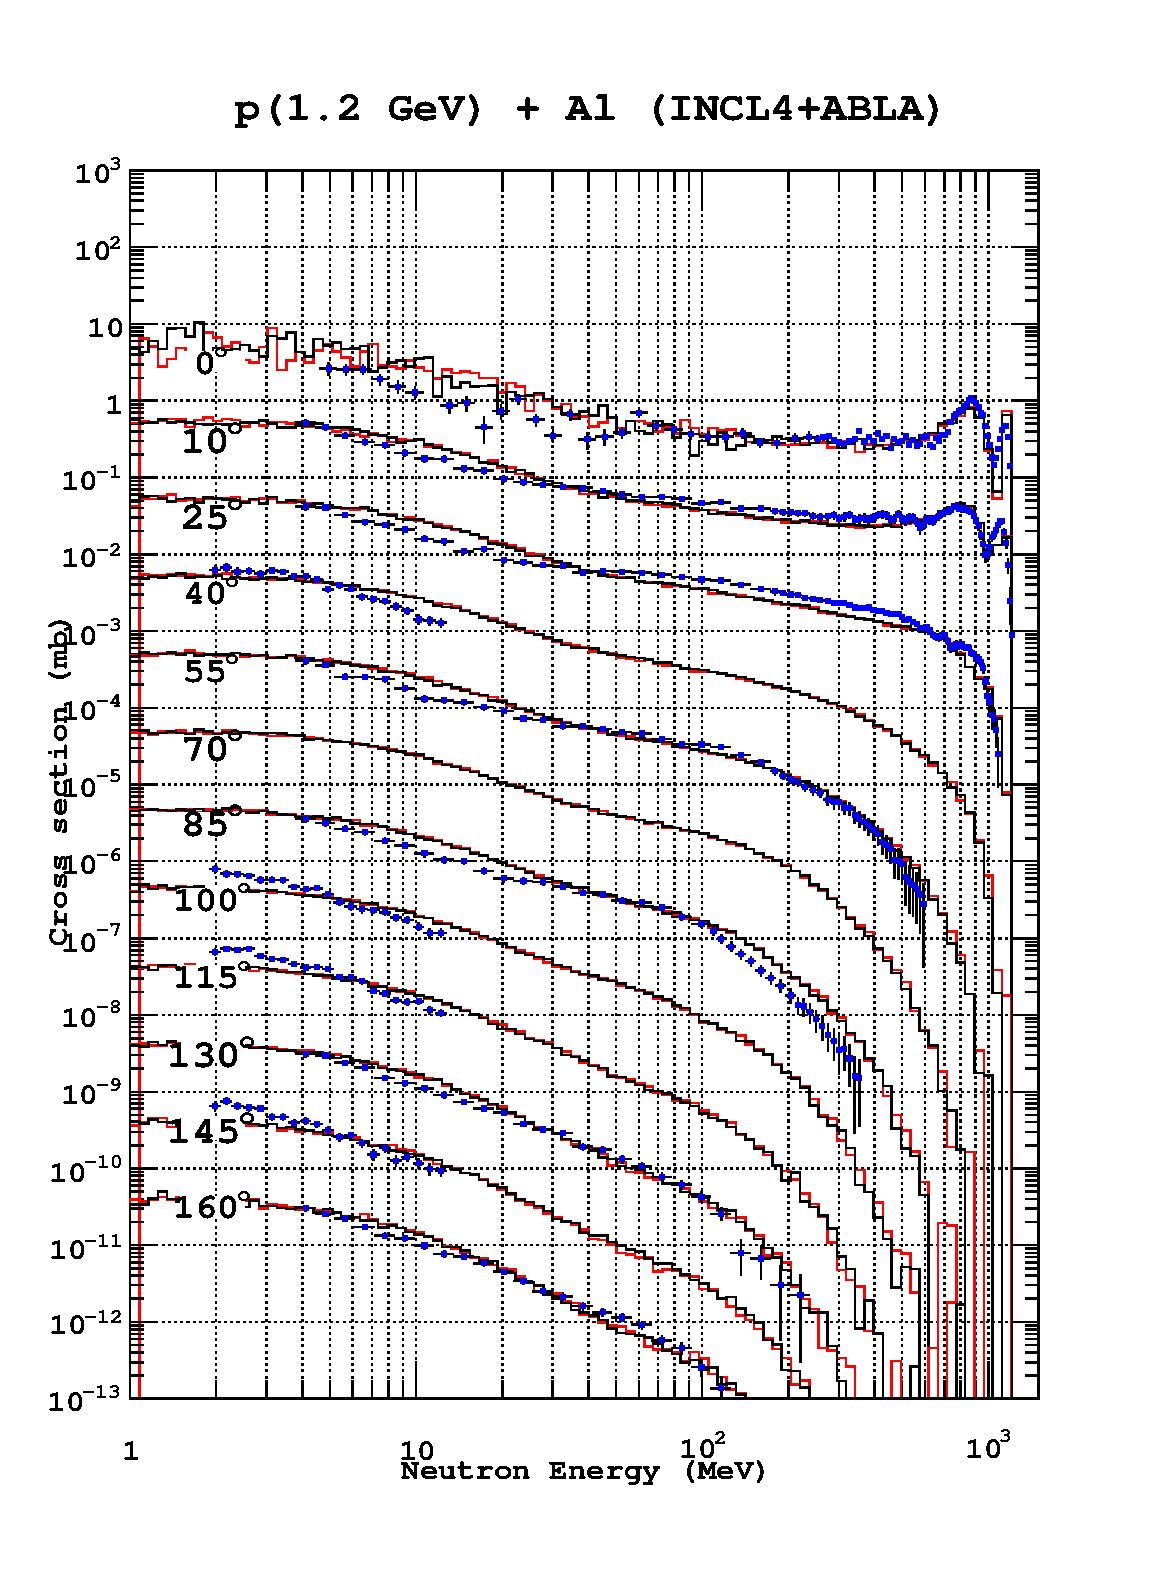
\includegraphics[scale=0.70]{images/proton1200MeVAl.eps}
\caption{\label{fig:neutronAl}Double-differential for neutron production cross section
    from Geant4 INCL and ABLA models in p(1.2 GeV) + Al $\rightarrow$ n + X reaction.
Histograms are the results from the original FORTRAN version (black) and new C++ implementation (red), respectively. 
Data is from Ref.~\cite{data}.}

\end{center}

\end{figure}


\begin{figure}
\begin{center}
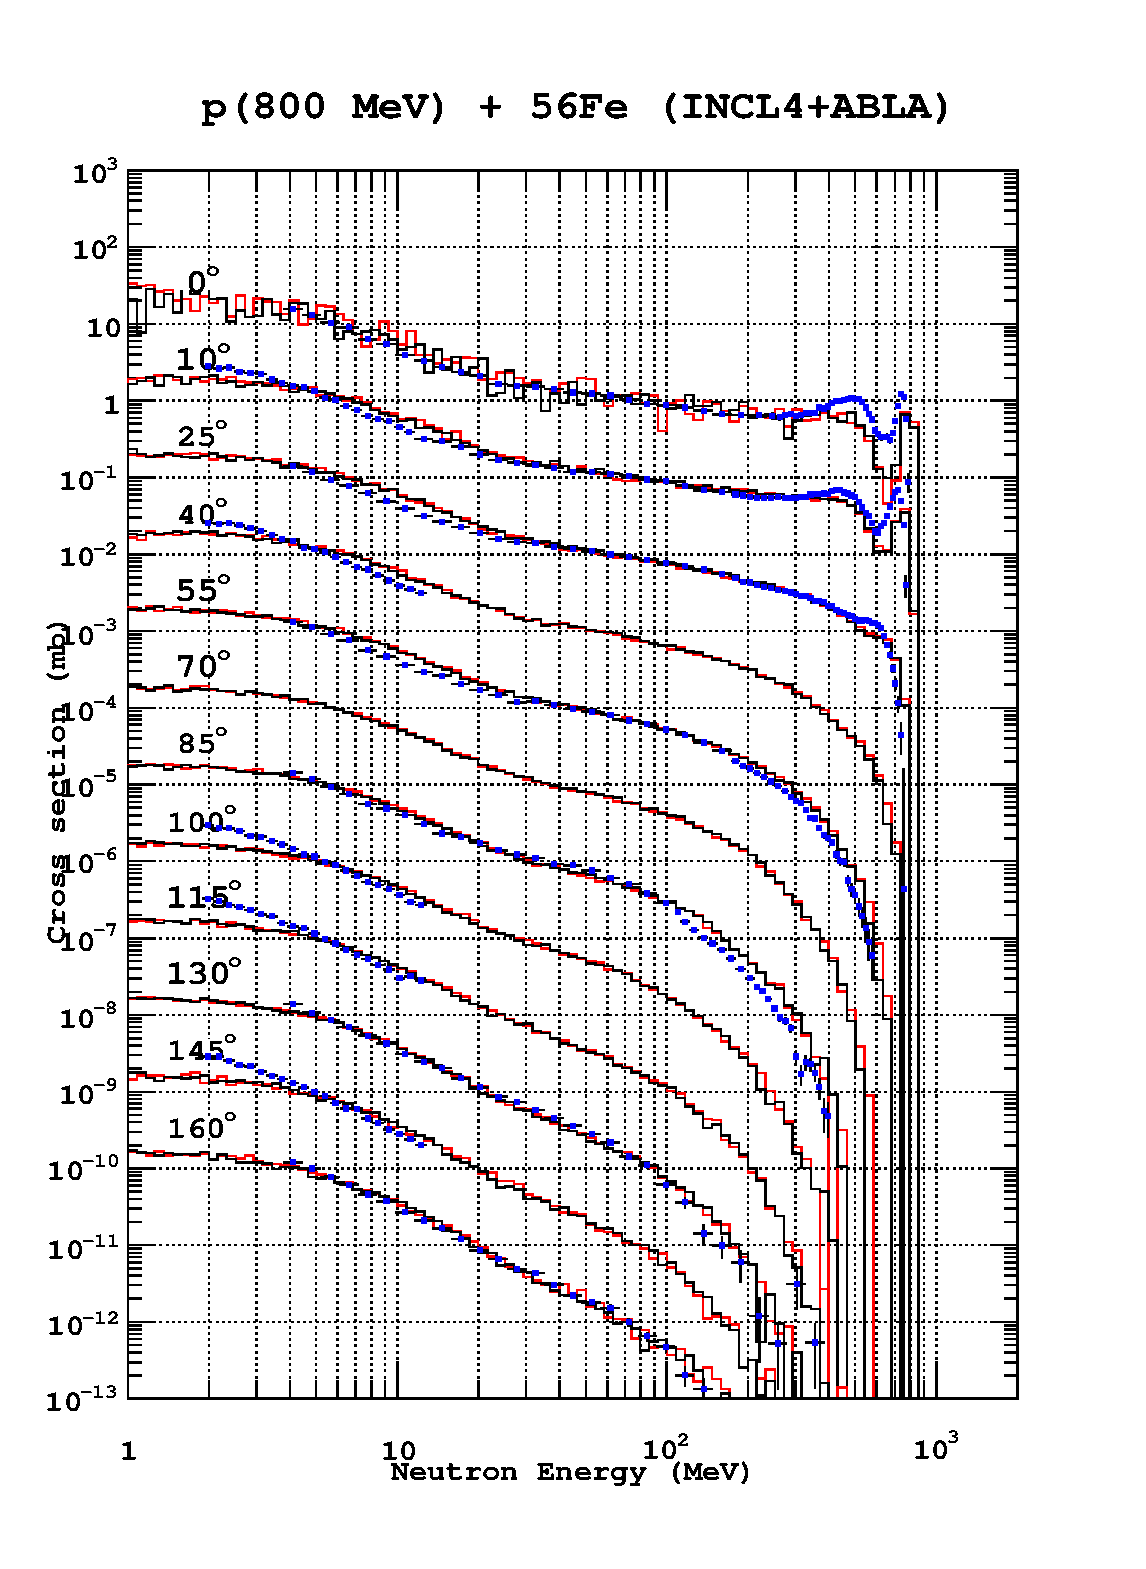
\includegraphics[scale=0.70]{images/proton800MeVFe.eps}
\caption{\label{fig:neutron08Fe}Neutron production from p(0.8 GeV) + Fe  $\rightarrow$ n + X. 
Data is from Ref.~\cite{data}.}
\end{center}

\end{figure}

\begin{figure}
\begin{center}
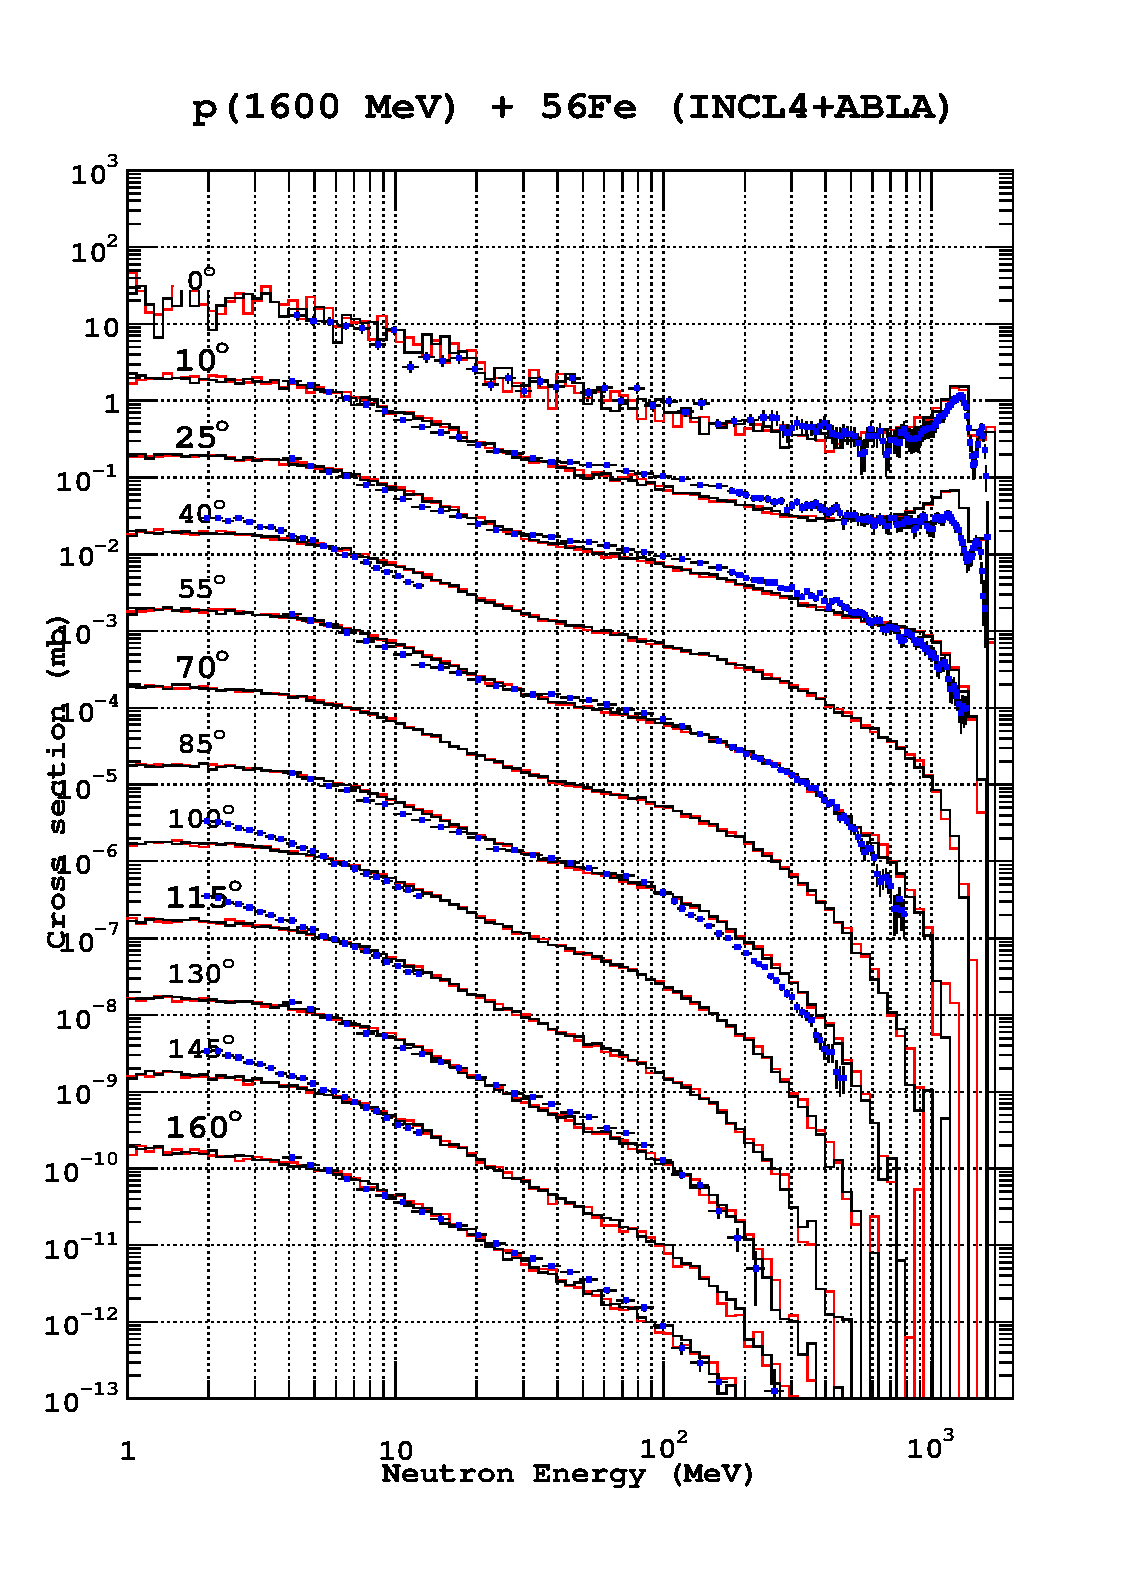
\includegraphics[scale=0.70]{images/proton1600MeVFe.eps}
\caption{\label{fig:neutronFe}Double-differential for neutron production cross section
    from Geant4 INCL and ABLA models in p(1.6~GeV) + Fe $\rightarrow$ n + X reaction.
Data is from Ref.~\cite{data}.}

\end{center}

\end{figure}

\begin{figure}
\begin{center}
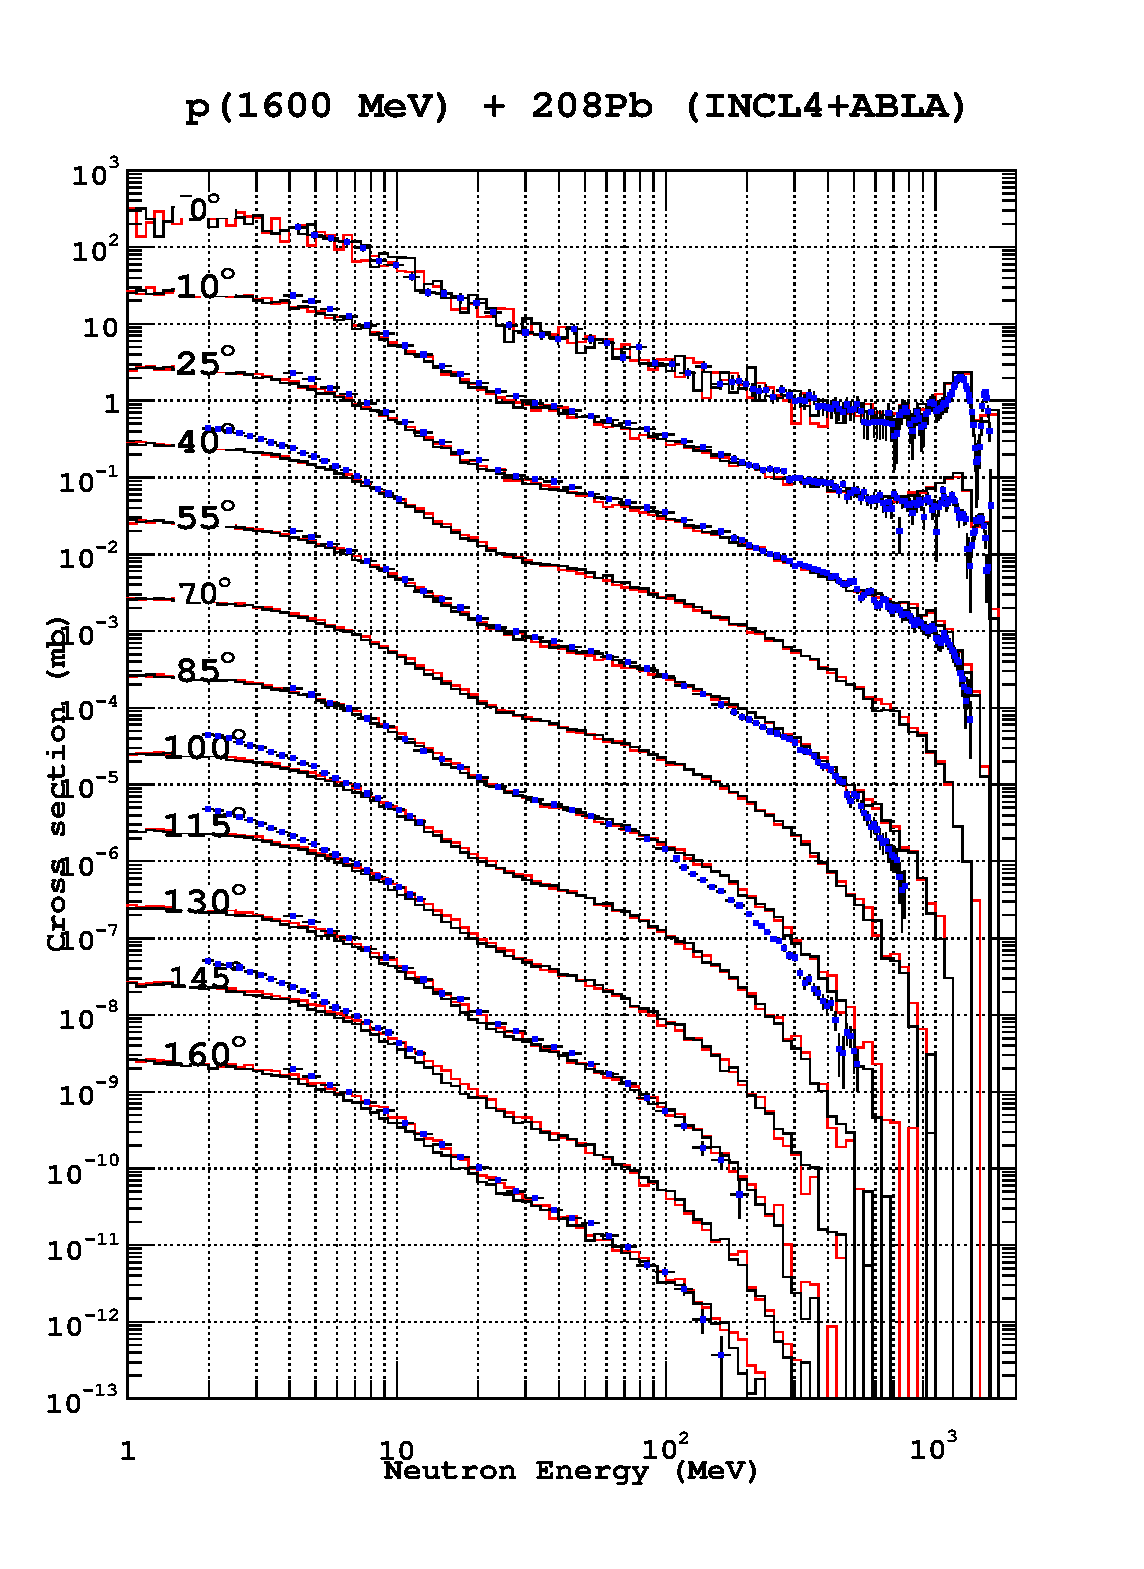
\includegraphics[scale=0.70]{images/proton1600MeVPb.eps}
\caption{\label{fig:neutronPb}Double-differential for neutron production cross section
    from Geant4 INCL and ABLA models in p(1.6~GeV) + Pb $\rightarrow$ n + X reaction.
Data is from Ref.~\cite{data}.}

\end{center}

\end{figure}

\section{Carbon projectiles}\label{sec:carbon}
The INCL4.2 method of handling composite projectiles is a simple extension 
of the single projectile particle case. 
Instead of shooting a single projectile particle an ion that consists of protons and neutrons is used.
Standard INCL4.2 implementation in Geant4 9.2 contains support for light ion projectiles 
up to $\alpha$ particle.

Carbon beams are of particular interest for medical applications of Geant4, 
and the method of composite projectiles has been used to extended INCL model to include carbon ions.
This functionality is already provided in Geant4 9.2 for interested test users, 
but more validation is needed before the formal release.
%and recently, a Carbon projectile support has been added to the INCL cascade. 

\section{Conclusion}\label{sec:conclusion}
The new Geant4 physics list {\tt QGSP\_\-INCL\_ABLA} for spallation studies 
provides powerful Geant4 machinery for ADS studies, enabling in an integrated fashion 
such diverse tasks as simulations of radioactive beams, 
electromagnetic interactions, and shielding studies. 
The power of this physics list comes from recent Geant4 implementations of 
dedicated  Fortran codes INCL4.2 and ABLA v3, providing detailed modelling
of spallation, fission, and evaporation.


Currently the physics models for the treatment of light ion beams needs to be improved and is underway.
%Ongoing work is the improvement of the physics models for the treatment of light ion beams.
In future releases the physics list {\tt QGSP\_\-INCL\_ABLA} will be further optimised. 
For low energy applications the physics list need to be modified
so that additional model is added below INCL/ABLA validity region to treat interactions of low energy particles.
Further, our goal is to completely redesign the INCL cascade code using modern object-oriented techniques
and taking benefit of the most recent INCL version \cite{inclTrieste}.

\ack %command \ack sets the acknowledgments heading as an unnumbered section.
We are grateful to INCL developers Joseph Cugnon (University of Li\'{e}ge, Belgium) and 
Y.~Yariv (SphN-DAPNIA, CEA-Saclay and Soreq, Israel) for supporting Geant4 INCL project.
The ABLA group kindly provided code to the Geant4 collaboration. 
Special thanks to Christelle Schmidt (IPNL) for providing a C++ translation of 
the ABLA fission model. 

%\appendix % The command \appendix" is used to signify the start of the appendixes.
%\section{AH:::}

%\begin{equation}
%time= money
%\end{equation}

%To obtain a simple heading of `Appendix' use the code \verb"\section*{Appendix}". 
%If it contains numbered equations, figures or tables the command \verb"\appendix" should
%precede it and \verb"\setcounter{section}{1}" must follow it. 


\section*{References}


\begin{thebibliography}{9}
\bibitem{geant4} Geant4 collaboration, 
\emph{Geant4 - a simulation toolkit}, Nucl. Instr. and Meth. A, 506, 2003, 250--303

\bibitem{eurisol}J.Cornell (ed.), \emph{The EURISOL Report, A feasibility study for a
European isotope-separation-on-line radioactive ion beam facility},
European Commission contract No. HPRI-CT-1999-50001, December 2003

\bibitem{ads}
C.~D. Bowman, \emph{Accelerator-driven systems for nuclear waste transmutation},
Annual Review of Nuclear and Particle Science Vol. 48: 505-556, December, 1998,
{\tt doi:10.1146/annurev.nucl.48.1.505}

\bibitem{incl} A. Boudard et al., \emph{Intra-nuclear cascade model for
    a comprehensive description of spallation reaction data}, Phys.
  Rev. C66 (2002) 044615

\bibitem{abla} J. Benlliure et al., \emph{Calculated nuclide
    production yields in relativistic collisions of fissile nuclei},
  Nuc. Phys. A628 (1998) 458

\bibitem{abla1} J. J. Gaimard et al., %\emph{},
  Nuc. Phys. A531 (1991) 709

\bibitem{abla2} A. R. Junghans et al., %\emph{},
  Nuc. Phys. A629 (1998) 635

\bibitem{g4site} Geant4 collaboration, {\tt http://\-cern.ch/\-geant4}

\bibitem{pk08bProceedings}
A. Heikkinen, P. Kaitaniemi, and A. Boudard,
{\em Implementation of INCL4 cascade and ABLA evaporation codes in Geant4},
Journal of Physics: Conference Series 119 (2008) 032024, {\tt doi:10.1088/1742-6596/119/3/032024}

\bibitem{doxygen} Doxygen source code documentation generator tool v1.5.9 (2009)

\bibitem{gsifragments} T. Enqvist et al. %\emph{},
  Nucl. Phys. A686 (2001) 481
\bibitem{g4incl} Geant4 collaboration, \emph{Geant4 9.2 Physics Reference Manual: INCL~4.2 Cascade and ABLA~v3 Evaporation with Fission} 
\bibitem{g4fermi} Geant4 collaboration, \emph{Geant4 9.2 Physics Reference Manual: Fermi Break-up Model} 
%\\ {\tt http://geant4.web.cern.ch/\-geant4/\-UserDocumentation/\-UsersGuides/\-PhysicsReferenceManual/\-html/\-node185.html}

\bibitem{data} S. Leray et al., \emph{Spallation Neutron Production by
  0.8, 1.2, and 1.6 GeV Protons on Various Targets} Phys. Rev. C65 044621 (1999)

\bibitem{inclTrieste} A. Boudard and J. Cugnon et al., \emph{Joint ICTP-IAEA Advanced Workshop on Model Codes for Spallation Reactions, page 29}, ICTP Trieste, Feb 2008

\bibitem{carbone}
D.L. Olson et al.,
{\em Factorization of fragment-production cross sections in relativistic heavy-ion collisions},
Phys. Rev. C28, 1602 (1983)
{\sf [doi:10.1103/PhysRevC.28.1602]}

%\bibitem{doxygen} \emph{Doxygen website} \\ {\tt http://\-www.doxygen.org/}
%\item Strite S and Morkoc H 1992 {\it J. Vac. Sci. Technol.} B {\bf 10} 1237 
\end{thebibliography}


\end{document}


